\documentclass[12pt,a4paper]{article}
\usepackage{datetime}
\usepackage{ragged2e}
\usepackage{graphicx}
\usepackage{subcaption}
\usepackage{mwe}
\usepackage{float}
\pagenumbering{gobble}
\begin{document}
\begin{center}
{\scshape\LARGE VIS-EUV Test Report \par}
{\scshape\Large \today, \currenttime \par}
\bigskip
{\scshape\large Grating Type:VIS \par}
{\scshape\large Grating Number:1 \par}
\end{center}
\noindent We are 98\% confident that the peak intensity...\\
\indent...for channel 1 lies at 7.3624 mm to a precision of 7.5 microns.\\
\indent...for channel 2 lies at 7.3613 mm to a precision of 7.7 microns.\\
\indent...for channel 3 lies at 7.362 mm to a precision of 7.3 microns.\\
\noindent The final model was created...\\
\indent...after 4 intensity scans.\\
\indent...with 10 measurements taken at each distance.\\
\indent...with data from 266 distances.\\
\begin{figure}[H]
\centering
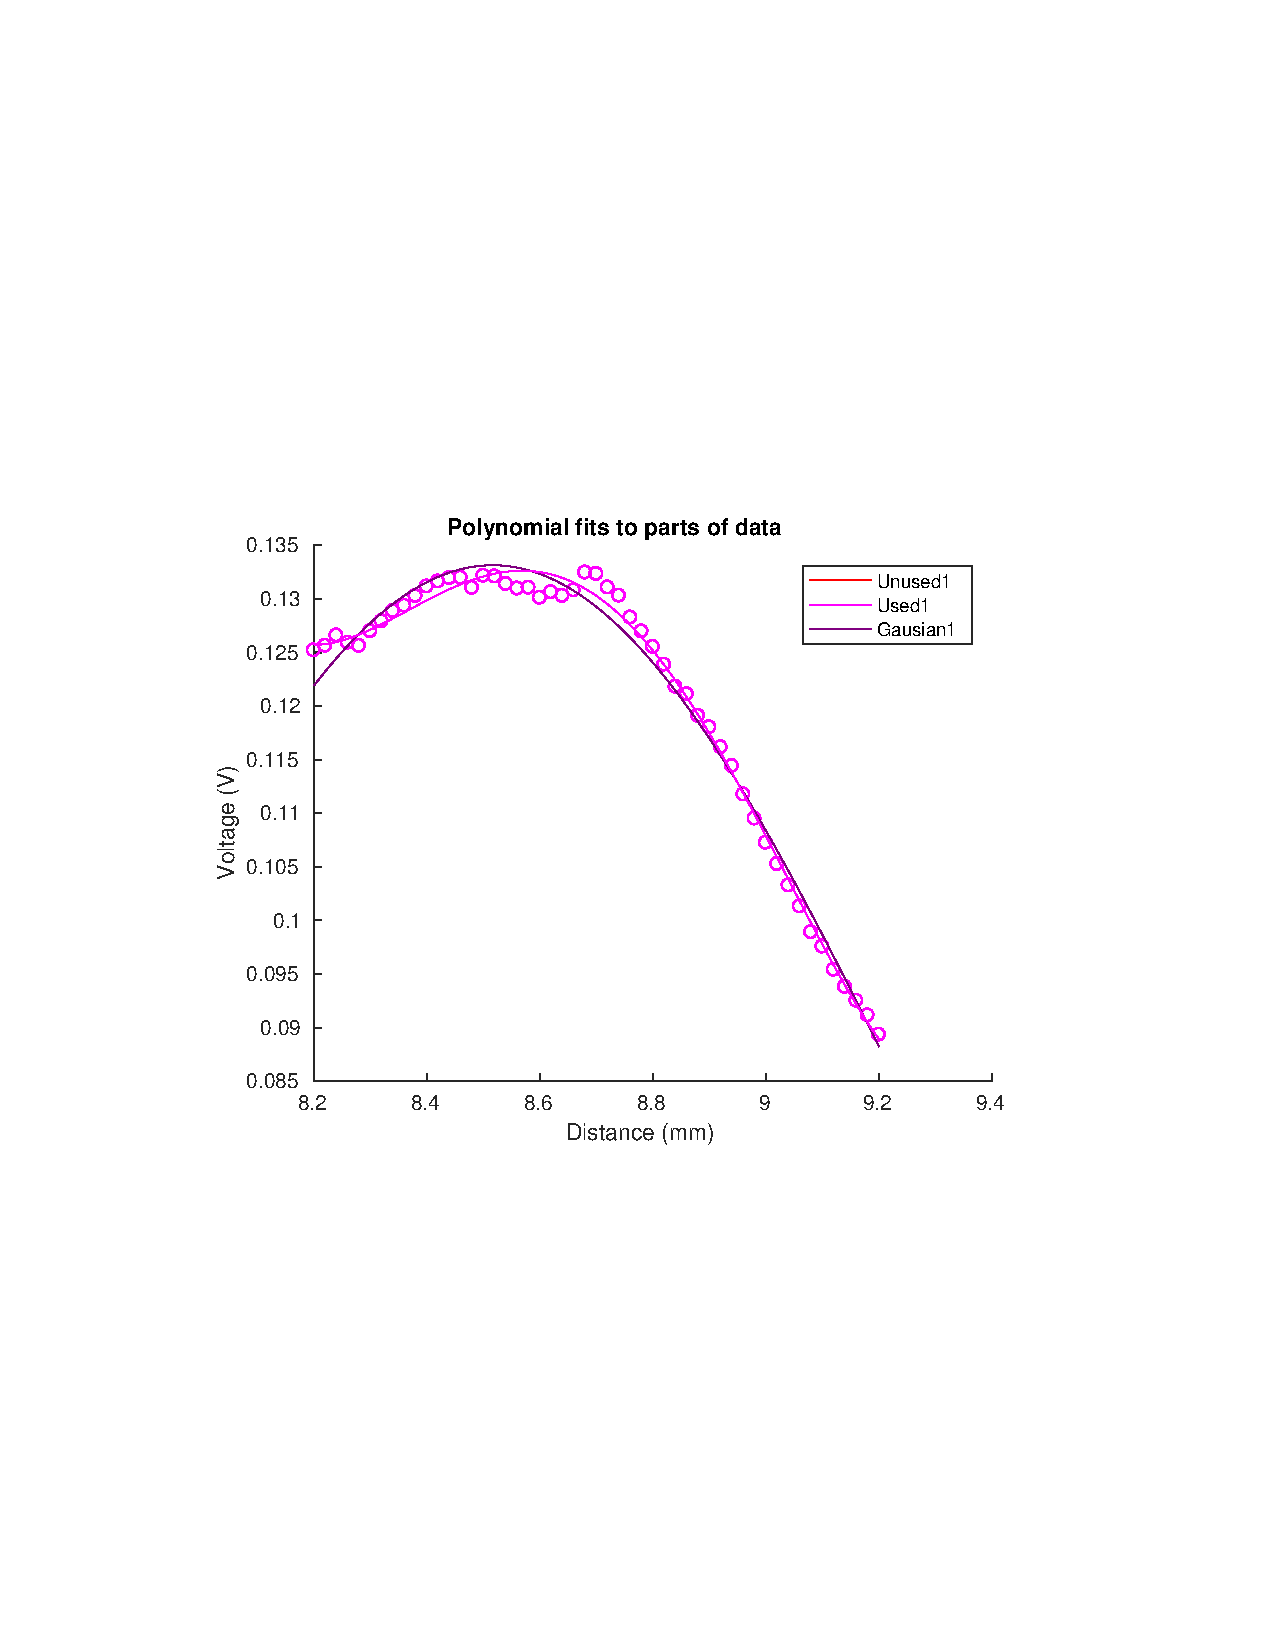
\includegraphics[height=.5\textheight, trim={4cm 8.5cm 4cm 8.5cm},clip]{/home/krg/ESIS/ESIS_VisEUV_transfer_sw/Output/VIS/grating_1/20170608-110415/iterations/iteration_3/all_fig_combo.pdf}\\
\end{figure}
\end{document}
